%Version 2.1 April 2023
% See section 11 of the User Manual for version history
%
%%%%%%%%%%%%%%%%%%%%%%%%%%%%%%%%%%%%%%%%%%%%%%%%%%%%%%%%%%%%%%%%%%%%%%
%%                                                                 %%
%% Please do not use \input{...} to include other tex files.       %%
%% Submit your LaTeX manuscript as one .tex document.              %%
%%                                                                 %%
%% All additional figures and files should be attached             %%
%% separately and not embedded in the \TeX\ document itself.       %%
%%                                                                 %%
%%%%%%%%%%%%%%%%%%%%%%%%%%%%%%%%%%%%%%%%%%%%%%%%%%%%%%%%%%%%%%%%%%%%%

\documentclass[sn-basic,pdflatex]{sn-jnl}

%%%% Standard Packages
%%<additional latex packages if required can be included here>

\usepackage{graphicx}%
\usepackage{multirow}%
\usepackage{amsmath,amssymb,amsfonts}%
\usepackage{amsthm}%
\usepackage{mathrsfs}%
\usepackage[title]{appendix}%
\usepackage{xcolor}%
\usepackage{textcomp}%
\usepackage{manyfoot}%
\usepackage{booktabs}%
\usepackage{algorithm}%
\usepackage{algorithmicx}%
\usepackage{algpseudocode}%
\usepackage{listings}%
%%%%

%%%%%=============================================================================%%%%
%%%%  Remarks: This template is provided to aid authors with the preparation
%%%%  of original research articles intended for submission to journals published
%%%%  by Springer Nature. The guidance has been prepared in partnership with
%%%%  production teams to conform to Springer Nature technical requirements.
%%%%  Editorial and presentation requirements differ among journal portfolios and
%%%%  research disciplines. You may find sections in this template are irrelevant
%%%%  to your work and are empowered to omit any such section if allowed by the
%%%%  journal you intend to submit to. The submission guidelines and policies
%%%%  of the journal take precedence. A detailed User Manual is available in the
%%%%  template package for technical guidance.
%%%%%=============================================================================%%%%

\usepackage{booktabs}
\usepackage{longtable}
\usepackage{array}
\usepackage{multirow}
\usepackage{wrapfig}
\usepackage{float}
\usepackage{colortbl}
\usepackage{pdflscape}
\usepackage{tabu}
\usepackage{threeparttable}
\usepackage{threeparttablex}
\usepackage[normalem]{ulem}
\usepackage{makecell}
\usepackage{xcolor}


\raggedbottom




% tightlist command for lists without linebreak
\providecommand{\tightlist}{%
  \setlength{\itemsep}{0pt}\setlength{\parskip}{0pt}}





\begin{document}


\title[]{Predicting Language Development among 12-month-old Infants From
Low-Income Families: A Machine Learning Approach based on
Socio-demographics Data at Birth}

%%=============================================================%%
%% Prefix	-> \pfx{Dr}
%% GivenName	-> \fnm{Joergen W.}
%% Particle	-> \spfx{van der} -> surname prefix
%% FamilyName	-> \sur{Ploeg}
%% Suffix	-> \sfx{IV}
%% NatureName	-> \tanm{Poet Laureate} -> Title after name
%% Degrees	-> \dgr{MSc, PhD}
%% \author*[1,2]{\pfx{Dr} \fnm{Joergen W.} \spfx{van der} \sur{Ploeg} \sfx{IV} \tanm{Poet Laureate}
%%                 \dgr{MSc, PhD}}\email{iauthor@gmail.com}
%%=============================================================%%

\author*[1]{\fnm{Hsuan-Wei} \spfx{(Isaac)} \sur{Chen} }\email{\href{mailto:hsuan-wei.chen@vanderbilt.edu}{\nolinkurl{hsuan-wei.chen@vanderbilt.edu}}}

\author[2]{\fnm{William} \spfx{R.} \sur{Doyle} }



  \affil*[1]{\orgdiv{Department of Psychology and Human
Development}, \orgname{Vanderbilt
University}, \orgaddress{\city{Nashville}, \country{USA}, \state{TN}}}
  \affil[2]{\orgdiv{Department of Leadership, Policy and
Organizations}, \orgname{Vanderbilt
University}, \orgaddress{\city{Nashville}, \country{USA}, \state{TN}}}

\abstract{Predicting language development among infants from low-income
families is crucial for later school success. This study uses machine
learning models, including elastic net and random forest, to predict
language development based on socio-demographic factors collected at
birth. Using a dataset from the Baby's First Years study designed to
examine the causal effects of unconditional cash transfers on early
development, our model was not able to achieve good predictive accuracy
(RMSE = 0.841). However, a few important predictors such as child sex
and household composition were identified and may provide implications
for supporting language development. This work contributes to
understanding how socio-demographic factors at birth influence language
development among infants from low-income families.}

\keywords{language, early childhood development, low-income
familites, machine learning}



\maketitle

\newgeometry{top=1in, bottom=1in, left=1in, right=1in}

\section{Introduction}\label{introduction}

\subsection{Problem Statement}\label{problem-statement}

Poverty and circumstances that give rise to it can significantly impact
a child's early development. Existing evidence suggest that children
from low-income backgrounds perform consistently below their
economically-advantaged peers on standardized language measures
(\citet{pace_identifying_2017}; \citet{romeo_language_2022}). However,
these studies have primarily focused on preschool children and these
associations are not indicative of causality. There remain many open
questions whether direct impacts on income can affect early childhood
development.

The Baby's First Years (BFY) study is randomized controlled trial (RCT)
that evaluates the causal impact of unconditional cash rewards on early
development of infants in low-income families. Data from this study
offer a unique opportunity to examine how socio-demographic factors
influence language development in infants from disadvantaged
backgrounds. In this study, we aim to leverage data from the BFY study
to predict early language development in infants of low-income mothers
using machine learning. Understanding how language develops among child
from low-income families is crucial because language abilities is a
strong predictor of later school readiness and success. Early
disparities in language development may translate to persistent gaps in
language ability that remain stable or widen over time.

\subsection{Motivation and Use Cases}\label{motivation-and-use-cases}

Accurate prediction of infant language development using
socio-demographic variables available at birth has wide-reaching
practical implications. First, early childhood programs and
developmental specialists can utilize the results of this research to
identify infants from low-income families that may benefit from
additional resources to support language development. In addition,
policy makers can use the results of this research to advocate for
unconditional cash transfer programs for low-income families. Above all,
families that gain access to resources and support systems as a result
of this work can help set their child up for future success from the
very start of life.

\section{Methods}\label{methods}

\subsection{Dataset Description}\label{dataset-description}

The BFY study is an ongoing RCT in the U.S. designed to evaluate the
causal impact of poverty reduction on a child's early development. Since
its initiation in 2018, the BFY has recruited 1,000 mothers of infants
with incomes below the federal poverty line across four diverse
communities: New York City, New Orleans, the greater Omaha metropolitan
area, and the Twin Cities of Minneapolis and St.~Paul. Mothers were
recruited from postpartum wards shortly after giving birth and received
a monthly cash gift by debit card for the first 76 months of their
child's life. Mothers were randomly assigned to one of two groups: (1)
an experimental group (n = 400) receiving \$333 per month (\$3,996 per
year) and (2) a control group (n = 600) receiving \$20 per month (\$240
per year). Importantly, participants did not lose eligibility to public
benefits (e.g.~Supplemental Nutrition Assistance Program, Head Start, or
Medicaid) due to the cash reward. Families in the BFY study were
involved in four waves of data collection. First, baseline data was
collected in the hospital shortly after birth. Afterwards, in-person
home visits were conducted when the child was 12 and 24 months of age.
Lastly, a university-based laboratory visit was conducted when the child
was 36 months of age (\citet{noble_babys_2021}).

The inclusionary criteria were as follows: (1) mother's self-reported
income was below the federal poverty threshold in the previous calendar
year; (2) mother was of legal age for informed consent; (3) infant was
admitted to the newborn nursery and not requiring admittance to the
intensive care unit; (4) mother was residing in the state of
recruitment; (5) mother reported not being ``highly likely'' to move to
a different state or country in the next 12 months; (6) infant was
discharged in the custody of the mother; and (7) mother was either
English or Spanish speaking (necessary for instruments of some child
outcomes) (\citet{noble_babys_2021}).

This analysis used self-reported surveys data collected at baseline
including mother demographics, mother-father relationship, and public
assistance as predictors of language outcome (\textbf{Table 1}). The
outcome of interest was the communication subscale of the Ages and
Stages Questionnaire, Third Editon (ASQ-3) collected at 12 months of
age. The ASQ-3 is a validated parental development screening
questionnaire designed to assess young children's progress across five
key domains: Communication, Gross Motor, Fine Motor, Problem Solving,
and Personal-Social. The communication domain specifically evaluates a
child's ability to understand and use of both expressive and receptive
language (e.g.~``Does your baby make two similar sounds, such as
`ba-ba', `da-da', or `ga-ga'?''). For each item, mothers reported the
frequency that their child exhibit the language skill (0 = not at all, 1
= sometimes, 2 = regularly). Item scores were summed to calculate total
raw scores and then were transformed into z-scores for analysis.

\begin{table}
\centering
\caption{\label{tab:table_1}Description of self-report survey measures and examples}
\centering
\fontsize{10}{12}\selectfont
\begin{tabular}[t]{ll}
\toprule
Measure & Survey Question Example\\
\midrule
Child Information & Child is female (Yes/No)\\
Mother Demographics & Mother's has unpaid maternity leave (Yes/No)\\
Father Demographics & Father's highest level of educaion attained (Multinomial)\\
Mother-Father Relationship & Biological dad put money towards baby's arrival (Yes/No)\\
Household Roster & Number of adults in the household including mother (Continuous)\\
Income/Net Worth & Household combined calculated income (Continuous)\\
Public Assistance & Household receives child care subsidy (Yes/No)\\
Maternal Health & Average alcohol drinks per week during pregnancy (Continous)\\
\bottomrule
\end{tabular}
\end{table}

\subsection{Dataset Access and
Cleaning}\label{dataset-access-and-cleaning}

The
\href{https://www.childandfamilydataarchive.org/cfda/archives/cfda/studies/37871/summary}{BFY}
dataset was downloaded from the Child and Family Data Archive (CFData)
platform. The CFData repository is maintained by Inter-university
Consortium for Political and Social Research at the University of
Michigan and is funded by the Office of Planning, Research, and
Evaluation. This platform hosts over 400 datasets on wide variety of
early care and education topics. Two Statistical Package for Social
Science (SPSS) data files from the BFY dataset were used for analysis:
the baseline dataset and age 1 dataset.

The two datasets were first combined and cleaned before subsequent
pre-processing steps. ASQ-3 communication scores were extracted from the
age 1 dataset and merged with the baseline dataset by subject ID.
Variables in the baseline data file are of two types -- raw and
generated. The raw variables were unprocessed, direct outputs the
self-reported surveys. The generated variables were created by BFY
analysts in preparation for data analysis. These variables were re-coded
(e.g., yes/no responses are coded yes = 1 and no = 0). In addition,
quality checks were conducted to create complicated generated variable.
For example, some mothers reported unexpectedly high household incomes,
and these mothers were recoded to the 99th percentile.

The merged dataset included 1,000 low-income mothers with newborns and
initially comprised of 627 features. After removal of raw variables, 169
features remained. Descriptive statistics of the mothers are presented
in \textbf{Table 2}. Prior to model training and tuning, a series of
preprocessing steps were conducted. Two models were trained for the
analyses: an elastic net model and a random forest model.

For the elastic net model, the data were pre-processed as follows: (1)
categorical levels constituting less than 1\% of the data were grouped
into an ``other'' category; (2) all categorical predictors were
dummy-coded; (3) predictors with more than 10\% missing data were
removed; (4) missing values in categorical predictors were imputed using
the training set mode; (5) missing values in numeric predictors were
imputed using the training set mean; (6) observations with missing
outcome values were removed; (7) predictors with zero variance were
removed; (8) predictors with a correlation above 0.95 with any other
predictor were removed; (9) all predictors were standardized to have a
mean of 0 and a standard deviation of 1.

For the random forest model, the data were pre-processed as follows: (1)
categorical levels constituting less than 1\% of the data were grouped
into an ``other'' category; (2) missing values in categorical predictors
were assigned to an ``unknown'' category; (3) all categorical variables
were dummy-coded; (4) observations with missing outcome values were
removed; (5) predictors with zero variance were removed.

\begin{table}
\centering
\caption{\label{tab:table_2}Descriptive statistics of mothers in the BFY study}
\centering
\fontsize{10}{12}\selectfont
\begin{tabular}[t]{lcc}
\toprule
\textbf{Characteristic} & \makecell[c]{\textbf{High Cash Gift}\ \ \\N = 400} & \makecell[c]{\textbf{Low Cash Gift}\ \ \\N = 600}\\
\midrule
\textbf{Age (years)} & 27.4 (5.9) & 26.8 (5.8)\\
\textbf{Race/Ethnicity} &  & \\
\hspace{1em}White & 34 (8.5\%) & 67 (11\%)\\
\hspace{1em}Black & 177 (44\%) & 237 (40\%)\\
\hspace{1em}Asian & 5 (1.3\%) & 4 (0.7\%)\\
\hspace{1em}Native & 1 (0.3\%) & 11 (1.8\%)\\
\hspace{1em}Multiple & 12 (3.0\%) & 24 (4.0\%)\\
\hspace{1em}Other & 5 (1.3\%) & 12 (2.0\%)\\
\hspace{1em}Hispanic & 166 (42\%) & 243 (41\%)\\
\textbf{Education Level} &  & \\
\hspace{1em}Less than high school diploma & 88 (22\%) & 147 (25\%)\\
\hspace{1em}High school diploma or GED & 207 (52\%) & 300 (50\%)\\
\hspace{1em}Some college, no degree & 68 (17\%) & 102 (17\%)\\
\hspace{1em}Associate's degree & 14 (3.5\%) & 19 (3.2\%)\\
\hspace{1em}Bachelor's degree or higher & 20 (5.0\%) & 31 (5.2\%)\\
\textbf{Household Combined Income} & 20,918 (16,146) & 22,466 (21,360)\\
\textbf{Maternal Depression (CEL-D)} & 7.0 (4.6) & 6.9 (4.5)\\
\bottomrule
\multicolumn{3}{l}{\rule{0pt}{1em}\textsuperscript{1} Mean (SD); n (\%)}\\
\end{tabular}
\end{table}

\section{Exploratory Analyses}\label{exploratory-analyses}

\subsection{Univariate Analyses}\label{univariate-analyses}

The distribution of z-scores for the ASQ-3 communication subscale is
presented in \textbf{Figure 1}. The distribution is left skewed with a
median {[}IQR{]} is 0.49 {[}-0.23 -- 0.99{]}. A total of 600 infants
scored greater than 1 SD below the mean, suggesting that their
development is on schedule. Sixty-three infants scored between 1 and 2
SD below the mean. These children may benefit from more language
activities and active monitoring on their developmental milestones. Ten
infants scores more than 2 SD below the mean and may need further
assessments with a professional.

\begin{figure}

{\centering 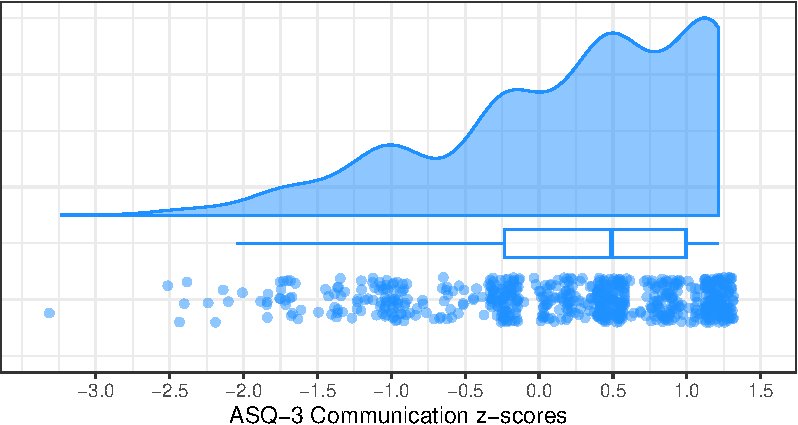
\includegraphics{HWC_final-paper-draft_files/figure-latex/fig_rain_ASQ-1} 

}

\caption{Raincloud plot of ASQ-3 z-scores in the communication domain. This plot utilizes three different plots to illustrate overall shape and variability: a half violin plot representing the kernel density estimate at the top, a boxplot showing the median and interquartile range at the center, and jittered individual data points at the bottom.}\label{fig:fig_rain_ASQ}
\end{figure}

\subsection{Bivariate Analyses}\label{bivariate-analyses}

The bivariate relationships between four demographic predictors and
ASQ-3 communication z-scores are depicted in \textbf{Figure 2}. The four
demographic predictors examined included treatment group, maternal
education, household combined income, and maternal depression. The bar
plot comparing treatment group and ASQ-3 communication z-scores
indicated that infants of mothers who received a high cash reward
demonstrated more age-appropriate language skills compared to infants of
mothers who received a low cash reward (\textbf{Figure 2A}). The bar
plot between maternal education and ASQ-3 communication z-scores did not
reveal any trend of age-appropriate language skills and maternal
education. (\textbf{Figure 2B}). The scatterplot comparing household
combined income and ASQ-3 communication z-scores appears to show a
positive relationship. However, the upward trend is primarily driven by
one outlier (\textbf{Figure 2C}). No linear or nonlinear trend was
observed in the scatterplot between maternal depression and ASQ-3
communication z-score (\textbf{Figure 2D}).

\begin{figure}

{\centering 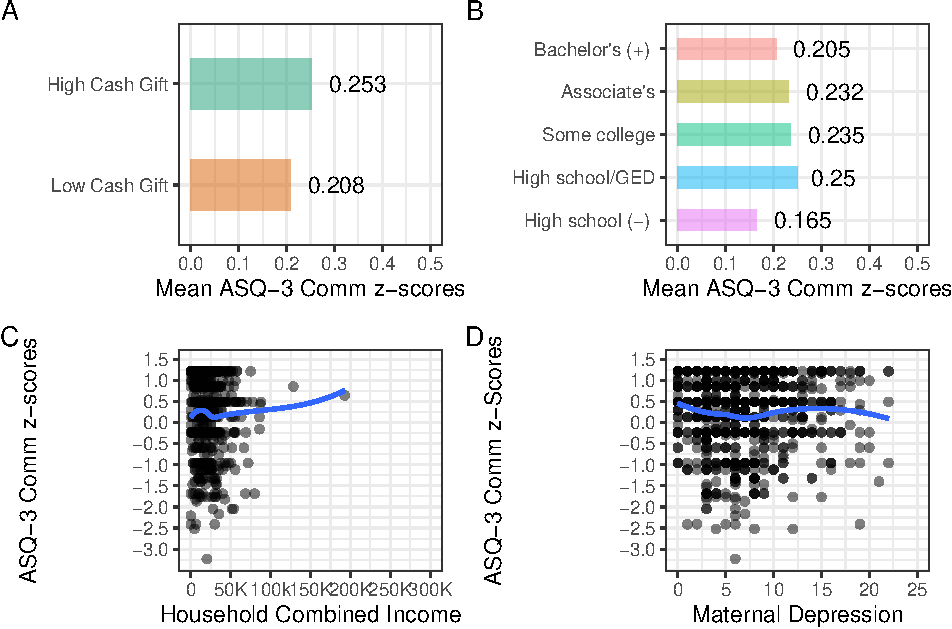
\includegraphics{HWC_final-paper-draft_files/figure-latex/fig_bivariate-1} 

}

\caption{(A) Bar plot of mean ASQ-3 communication z-scores by mothers who received a high cash reward versus a low cash reward. (B) Bar plot of mean ASQ-3 communication z-scores by different levels of maternal education. Bachelor's (+) represents Bachelor's degree or higher. High school (-) represents less than high school. (C) Scatter plot of ASQ-3 communication z-scores as a function of household combined income. (D) Scatter plot of ASQ-3 communication z-scores as a function of maternal depression. Maternal depression was measured by the Center for Epidemiologic Studies Depression Scale (CES-D). A loess curve was fitted to each scatterplot.}\label{fig:fig_bivariate}
\end{figure}

\section{Model Development}\label{model-development}

\subsection{Model Selection}\label{model-selection}

The current dataset is characterized by a relatively low number of cases
(\textless{} 2,000) and a relatively high number of features
(\textgreater{} 50). Given these characteristics, two models were
selected for analysis: an elastic net model and a random forest model.
An elastic net model was chosen for its ability to handle datasets with
smaller sample sizes, compared to models such as XGBoost or neural nets
that require larger sample sizes. Moreover, elastic net combines both L1
(lasso) and L2 (ridge) regularization to simultaneously shrink
coefficients and perform variable selection, making it a versatile
approach for datasets with many features. Elastic net models also
produce more interpretable results.

Although random forest models generally perform better with larger
sample sizes, this model was chosen for analysis for several reasons.
First, a random forest model can effectively handle datasets with a
large number of features and can capture complex nonlinear relationships
between predictors. The model is also robust to missing data and can
even incorporate it during training. Lastly, random forests require
minimal preprocessing of data and does not make assumptions about data
distribution.

\subsection{Hyperparameter Tuning}\label{hyperparameter-tuning}

To train and tune the elastic net model, cross-validation was performed
using a Monte Carlo resampling approach with 1,000 iterations to obtain
more reliable performance estimates. In each resample, 75\% of the data
was randomly chosen without replacement to train the model, while the
remaining 25\% served as the validation set. A regular grid search was
conducted across 20 levels for each of the two key hyperparameters:
mixture, which determines the balance between L1 and L2 regularization;
and penalty, which determines the overall strength of regularization.
For each resample, elastic net models were fitted across 400 (20x20)
combinations of penalty and mixture. Model performance was evaluated
using root mean squared error (RMSE) on the validation data. Final model
selection was based on the combination of penalty and mixture yielding
the lowest average RMSE across resamples.

For the random forest model, cross-validation was similarly performed
using a Monte Carlo resampling approach, but with 100 iterations. In
each resample, 75\% of the data was randomly selected for training, and
25\% for validation. Each random forest consisted of 100 trees. A
regular grid search was implemented across 10 levels for two key
hyperparameters: mtry, the number of predictors randomly sampled at each
split (ranging from 10 to 150); and min\_n, the minimum number of
observations needed to keep splitting nodes. For each resample, the
random forest models were fitted across 100 (10x10) combinations of mtry
and min\_n values. Model performance was evaluated using RMSE on the
validation data. Final model selection was based on the combination of
mtry and min\_n values yielding the lowest average RMSE across
resamples.

\begin{figure}

{\centering 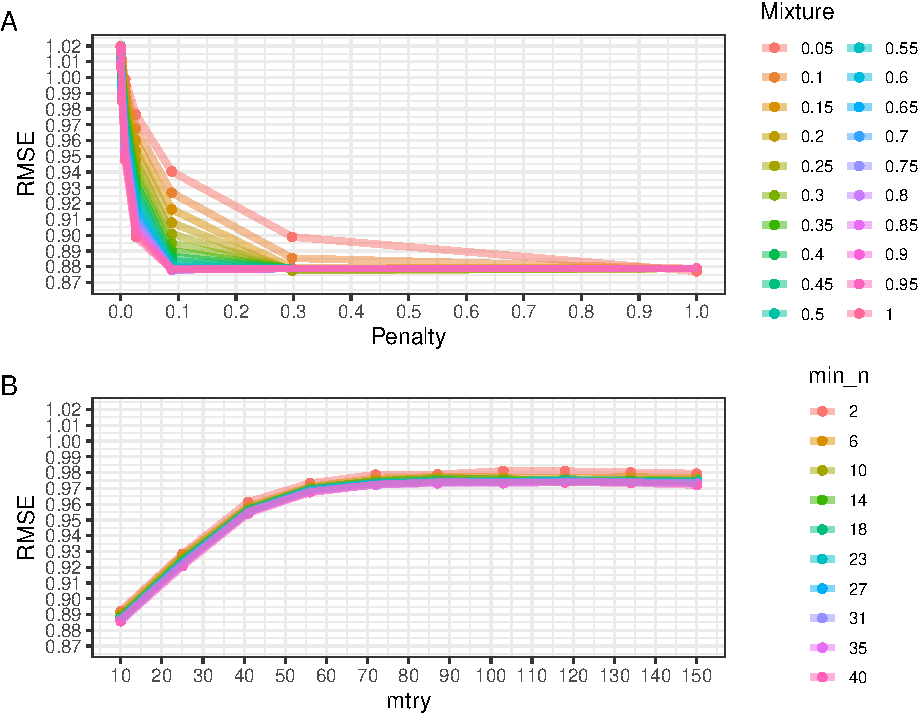
\includegraphics{HWC_final-paper-draft_files/figure-latex/fig_hyperparameter_performance-1} 

}

\caption{(A) Line plot of elastic net model performance across multiple hyperparameter combinations. (B) Line plot of random forest model performance across multiple hyperparameter combinations.}\label{fig:fig_hyperparameter_performance}
\end{figure}

Visualizations of model performance for the elastic net and random
forest models across multiple hyperparameter combinations are shown in
\textbf{Figure 3}. Results of tuning process for the elastic net model
indicated that model performance is generally better at higher values of
penalty. Higher mixture values also lead to improved model performance.
The elastic net model that yielded the best model performance (RMSE =
0.877) during training had a penalty value of 1 and mixture value of
0.05 (\textbf{Figure 3A}). Results of the tuning process for the random
forest model revealed that smaller values of mtry and larger values of
min\_n optimized model performance. The random forest model that yielded
the best model performance (RMSE = 0.886) during training had a mtry
value of 10 and min\_n value of 40 (\textbf{Figure 3B}). These results
suggest that the elastic net model performed better than the random
forest model during training.

\section{Model Performance}\label{model-performance}

\subsection{Evaluation on Held-out Testing Set between
Models}\label{evaluation-on-held-out-testing-set-between-models}

A quarter of the initial dataset was reserved as the testing set. The
elastic net model yielded a RMSE value of 0.841 on the testing set using
the combination of best hyperparameters (penalty = 1; mixture = 0.05).
The random forest model yielded a RMSE value of 0.853 using the
combination of best hyperparameters (mtry = 2; min\_n = 40). This result
suggests that the elastic net model performed better than the random
forest model and will be used as the final model for predicting language
development among infants of low-income parents.

\section{Final Model Interpretation}\label{final-model-interpretation}

\subsection{Characteristics of Final
Model}\label{characteristics-of-final-model}

The final elastic net model was fitted to predict standardized ASQ-3
communication scores using 110 predictors. The model used a penalty
value of 1 and a mixture vale of 0.05. Given the regular grid search
only assessed penalty values between 0 and 1, selection of the highest
penalty value indicates that strong regularization was important for
optimizing model performance. The low mixture value positioned the model
close to ridge regression while allowing for limited variable selection.
Variable estimates extracted from the final model revealed that only 16
predictors retained non-zero coefficients. This result may suggest that
most predictors in the dataset were weak predictors of language
development; and the combination of strong regularization and a small
lasso component contributed to the exclusion of those variables. In
addition, the results indicate that a parsimonious model can achieve
good model performance.

\begin{figure}

{\centering 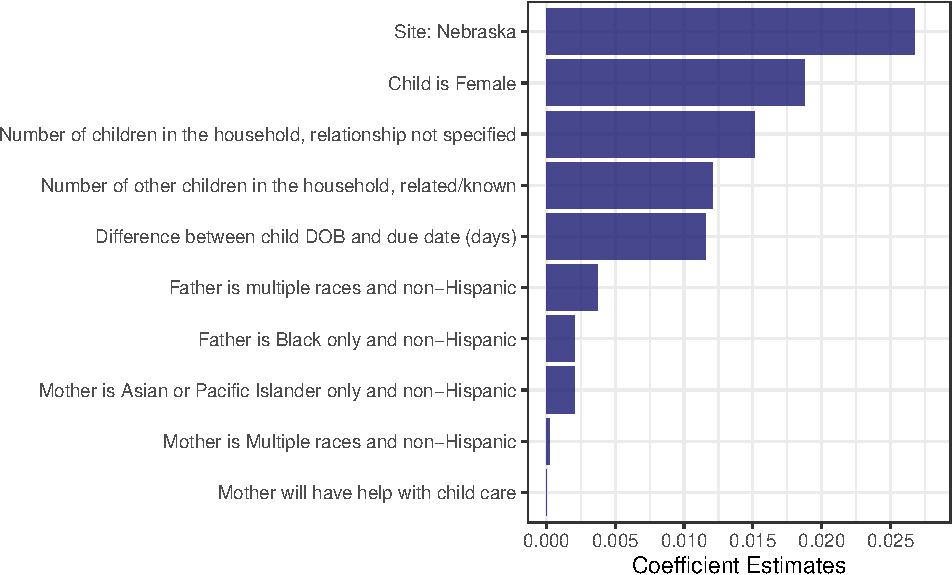
\includegraphics{HWC_final-paper-draft_files/figure-latex/fig_bar_enet_vi-1} 

}

\caption{(A) Bar plot of coefficient estimate magnitudes for the elastic net model. (B) Bar plot of variable importance for the random forest model. DOB = Date of Birth.}\label{fig:fig_bar_enet_vi}
\end{figure}

However, the RMSE for the final model was 0.841 for predicting ASQ-3
communication z-scores. This result indicates that the model's
predictions deviate by 0.841 SDs from the actual values and does not
reflect good model performance. The 10 predictors with the largest
coefficient magnitudes are shown in \textbf{Figure 4}. The most
important predictors of ASQ-3 communication z-scores were whether data
collection occurred in Omaha, Nebraska, the child's sex, and the number
of children in the household.

\section{Implications and Use Cases
Revisited}\label{implications-and-use-cases-revisited}

\subsection{Applications in Practice}\label{applications-in-practice}

Although the final model demonstrated poor predictive performance and is
not recommended for deployment, the variables identified as important
may still offer valuable insights. For example, the elastic net model
highlighted child sex as a key predictor. This suggests that parents and
developmental specialists might consider providing additional language
activities for boys to support their early language development.
Furthermore, the number of children in the household emerged as another
important factor. Infants living without other children in the household
may benefit from increased frequency of social interaction with peers to
promote language skills.

\subsection{Limitations and Future
Work}\label{limitations-and-future-work}

Several limitations should be considered when interpreting the findings
of this study. First, the analysis was restricted to socio-demographic
variables collected at birth. Given that language development is shaped
by social interactions and environmental factors, variables measured
after birth, such as home literacy environment or frequency of peer
interactions may be stronger predictors of language outcomes.
Additionally, the current analysis did not include interaction terms and
may have potentially overlooked important moderating effects among
socio-demographic factors. Future work could apply causal machine
learning approaches to better understand the effects of unconditional
cash transfers on language development. Exploring alternative
hyperparameter optimization strategies, such as Bayesian optimization or
simulated annealing, may also improve model performance.

~

\bibliography{bibliography.bib}


\end{document}
